\appendix
\section{Goniometrické funkce}\label{appa}

\begin{figure}[ht!]
     \centering
     \begin{subfigure}{0.26\textwidth}
         \centering
         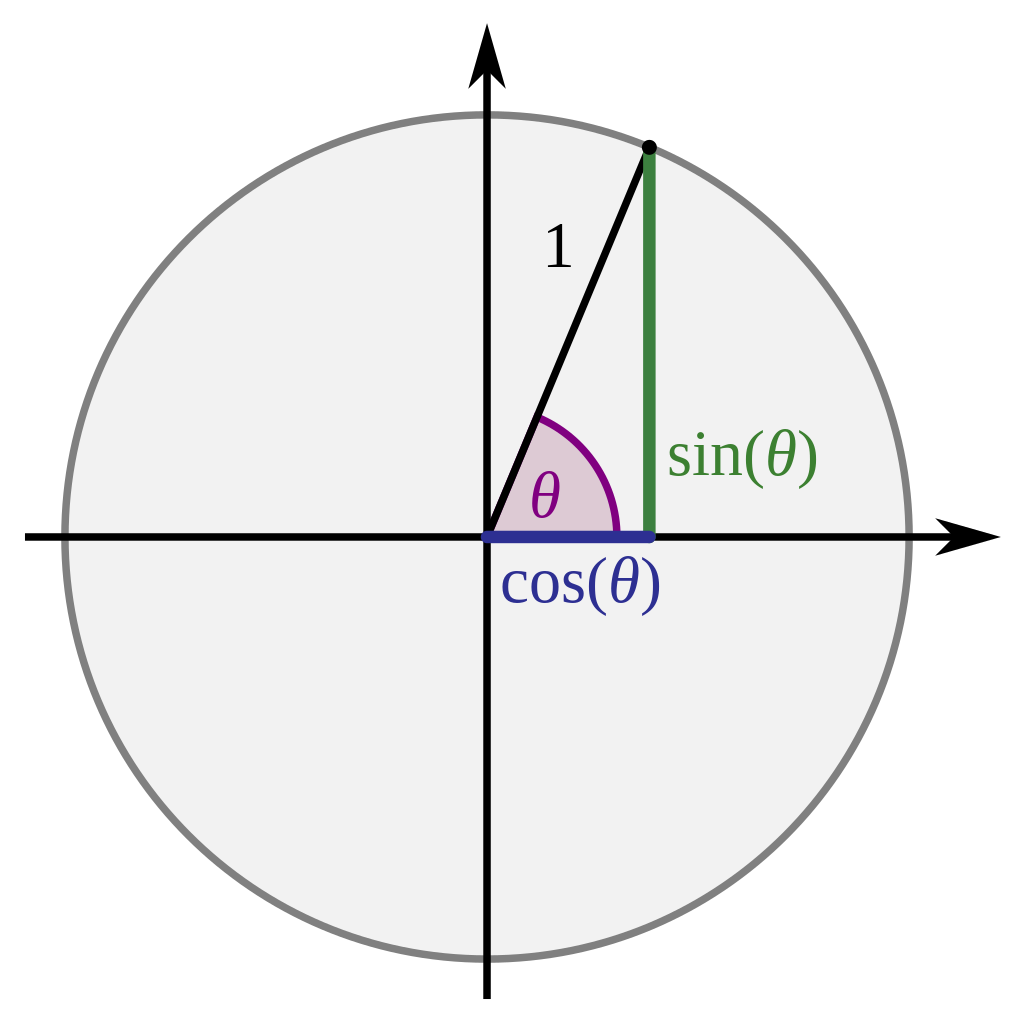
\includegraphics[width=\linewidth]{jednotkova_kruznice.png}
         \caption{Jednotková kružnice}
     \end{subfigure}
     \begin{subfigure}{0.65\textwidth}
         \centering
         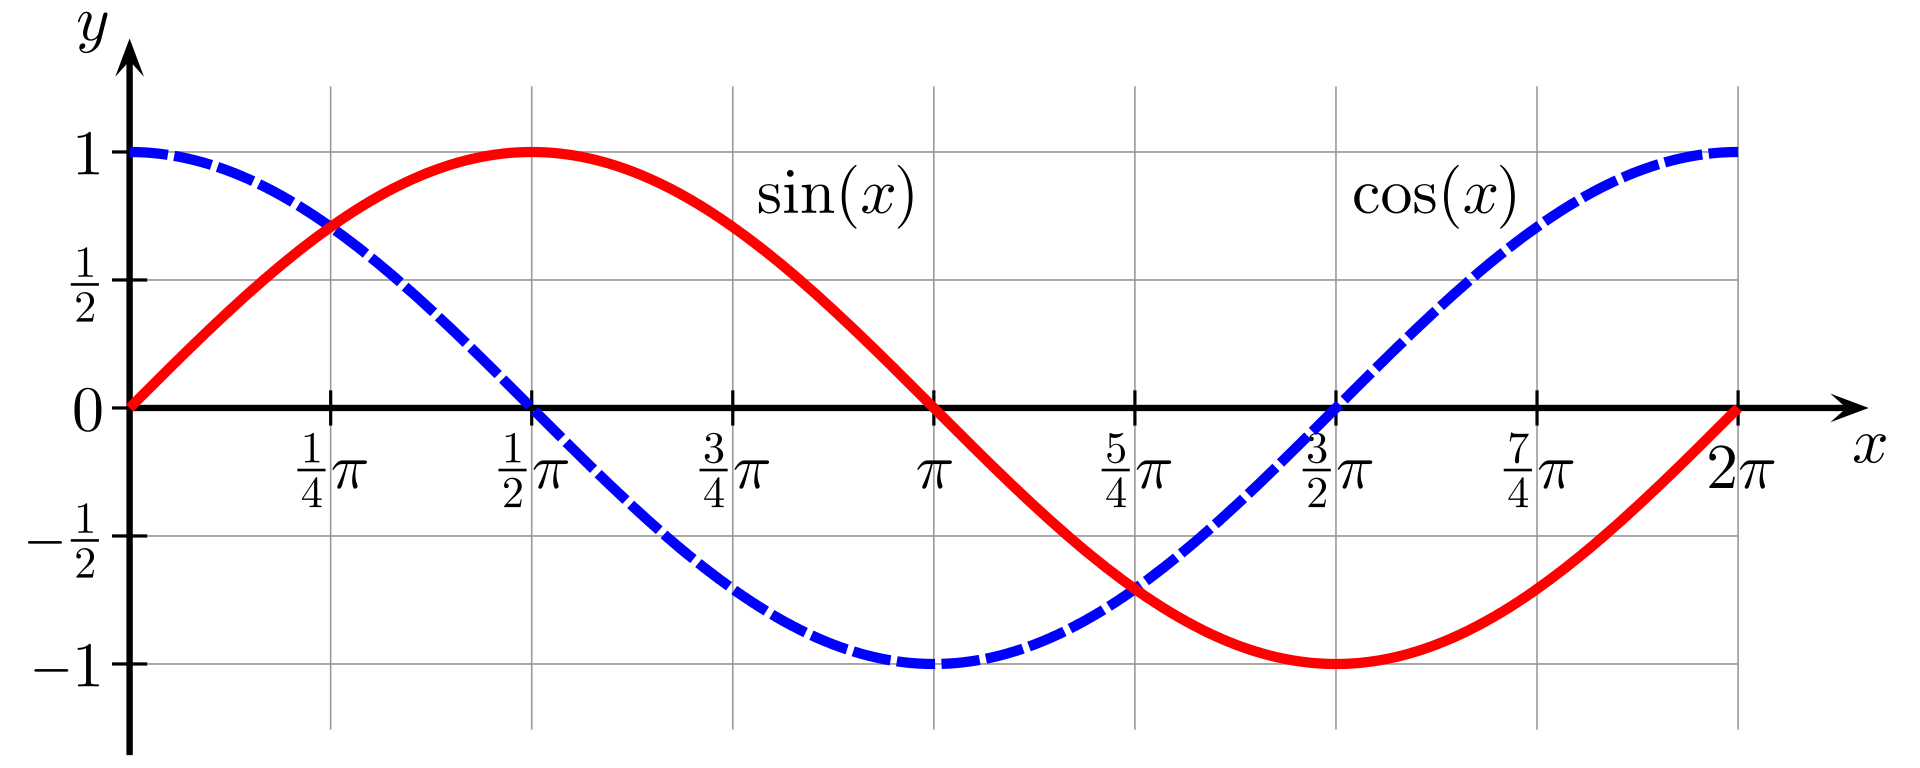
\includegraphics[width=\linewidth]{prubeh.png}
         \caption{Průběh funkcí $\sin$ a $\cos$}
     \end{subfigure}
     \caption{Funkce $\sin$ a $\cos$}
\end{figure}

\begin{figure}[ht!]
     \centering
     \begin{subfigure}{0.49\textwidth}
         \centering
         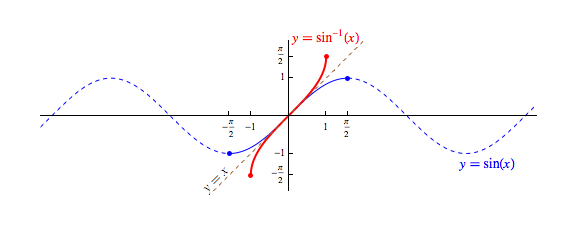
\includegraphics[width=\linewidth]{arcsine.png}
         \caption{Průběh funkce $\arcsin$}
     \end{subfigure}
     \begin{subfigure}{0.49\textwidth}
         \centering
         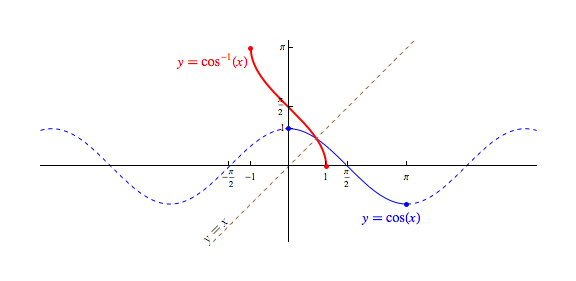
\includegraphics[width=\linewidth]{arccosine.png}
         \caption{Průběh funkce $\arccos$}
     \end{subfigure}
     \caption{Funkce $\arcsin$ a $\arccos$}
\end{figure}

\begin{figure}[ht!]
     \centering
     \begin{subfigure}{0.49\textwidth}
         \centering
         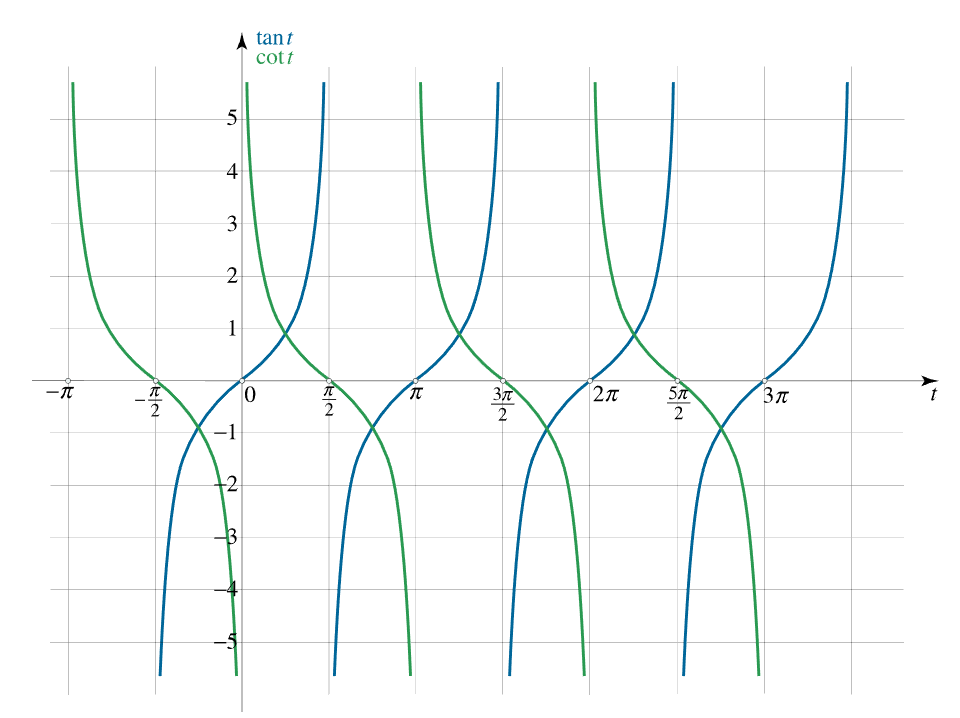
\includegraphics[width=\linewidth]{tgcotg.png}
         \caption{Průběh funkce $\tg$ a $\cotg$}
     \end{subfigure}
     \begin{subfigure}{0.49\textwidth}
         \centering
         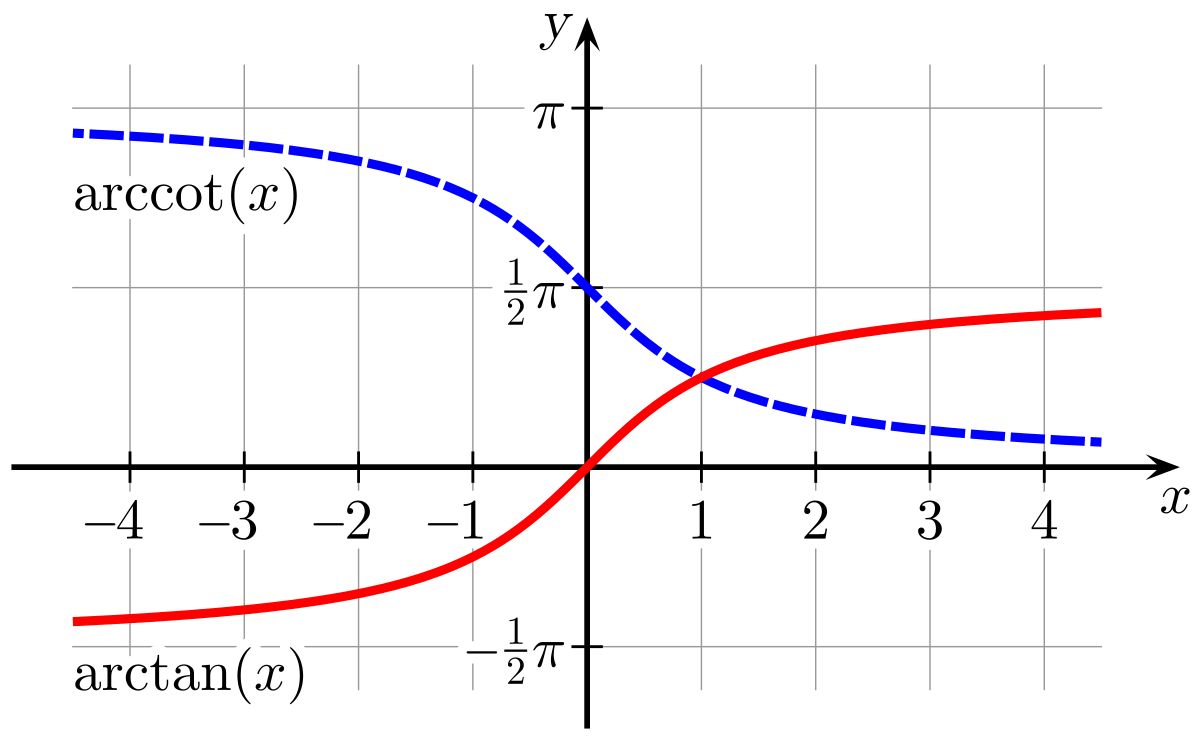
\includegraphics[width=\linewidth]{arctg_arccotg.png}
         \caption{Průběh funkce $\arctg$ a $\arccotg$}
     \end{subfigure}
     \caption{Funkce $\tg$ a $\cotg$}
\end{figure}

\begin{figure}[ht!]
     \centering
     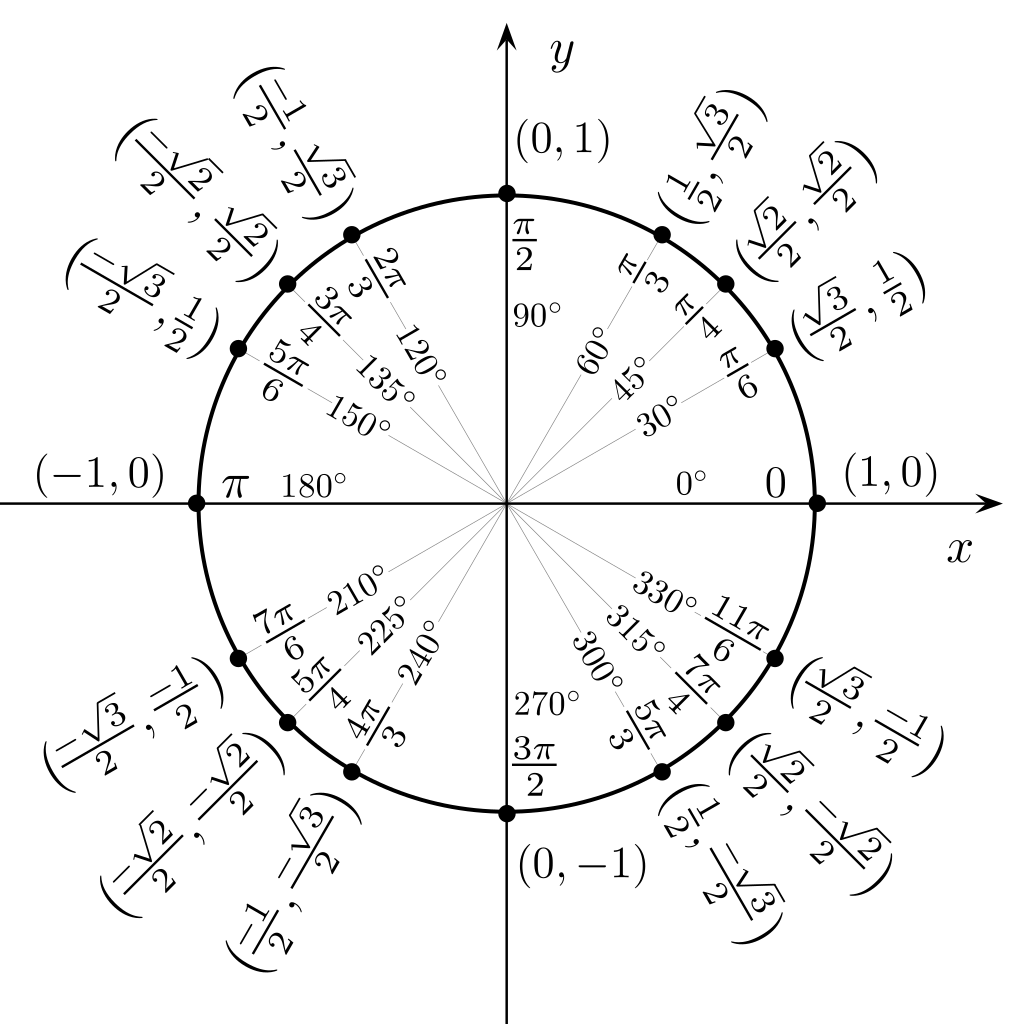
\includegraphics[width=0.6\linewidth]{jedn_k_s_hodn.png}
     \caption{Jednotková kružnice s hodnotami $(\cos \varphi, \sin \varphi)$}
     \label{kruzsh}
\end{figure}

\begin{figure}[ht!]
     \centering
     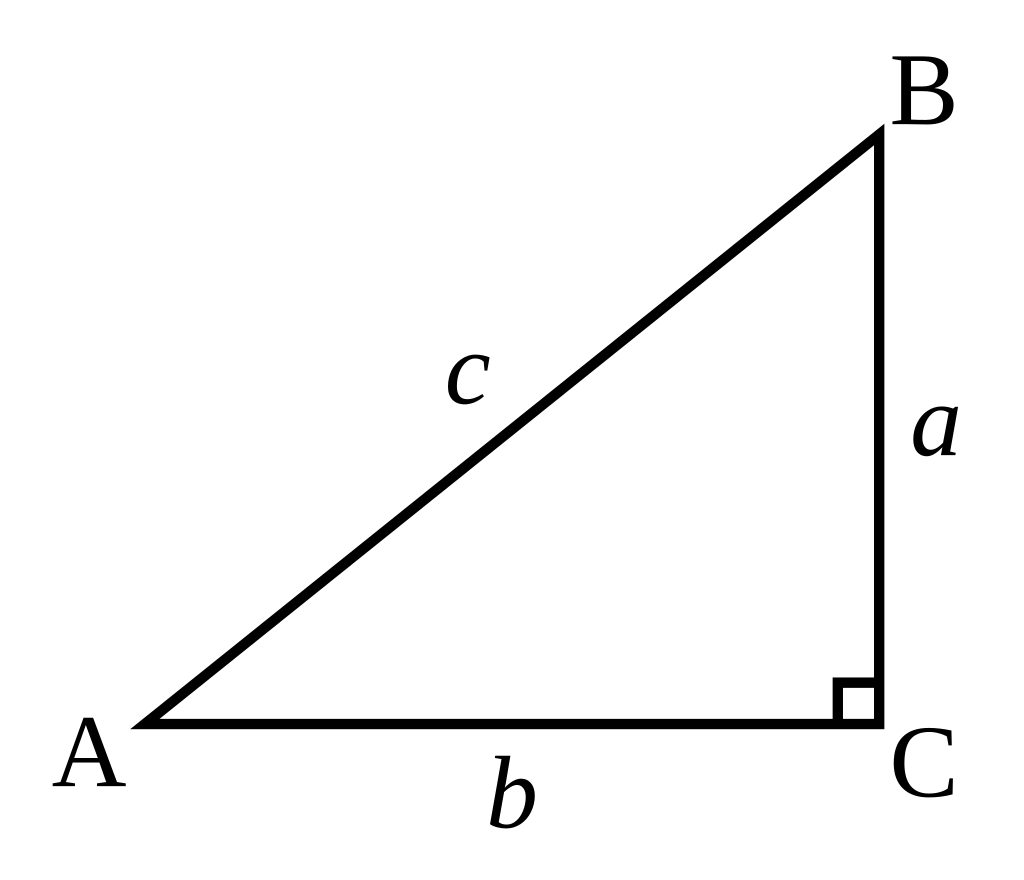
\includegraphics[width=0.3\linewidth]{right_t.png}
     \caption{Pravoúhlý trojúhelník s přeponou $c$}
     \label{prav_t}
\end{figure}

\pagebreak

\begin{pozn}
    \par V obrázku \ref{kruzsh} jsou uvedeny hodnoty funkcí sinus a kosinus ve tvaru
    komplexního čísla, víme totiž
    $$ a = | a | \cdot (\cos \varphi + i\mkern1mu \sin \varphi)$$
    pro nějaké $a \in \mathbb C.$ Jelikož se jedná o jednotkovou kružnici, kde platí
    $|a| = 1,$ máme
    $$a=\cos \varphi +i\mkern1mu \sin \varphi. $$
    Pokud chápeme komplexní číslo jako uspořádanou dvojici $(k,l)=k+i\mkern1mu l,$
    dobereme se k~zápisu, jenž je použit v obrázku.
    \par Všimněme si navíc, že platí
    $$k^2+l^2=1 \,\,\,\,\,\, \forall (k,l).$$
\end{pozn}

\begin{pozn}
    V obrázku \ref{prav_t} platí pro úhel $\alpha = \sphericalangle BAC:$
    \begin{enumerate}[$i.$]
        \item $\sin \alpha= \frac{a}{c},$
        \item $\cos \alpha= \frac{b}{c},$
        \item $\tg \alpha= \frac{a}{b},$
        \item $\arctg \alpha= \frac{b}{a}.$
    \end{enumerate}
\end{pozn}

\begin{pozn}[Základní hodnoty goniometrických funkcí]\,\\
    \begin{tabularx}{\textwidth}{| p{0.087\textwidth} || p{0.081\textwidth} | p{0.081\textwidth} |
    p{0.081\textwidth} | p{0.081\textwidth} | p{0.081\textwidth} | p{0.081\textwidth} | p{0.081\textwidth}
    | p{0.081\textwidth} |}
    \hline
    $\beta$ [$^\circ$] & 0 & 30 & 45 & 60 & 90 & 180 & 270 & 360 \\
    \hline
    $\alpha$ [rad] & 0 & $\frac{\pi}{6}$ & $\frac{\pi}{4}$ & $\frac{\pi}{3}$ & $\frac{\pi}{2}$ & $\pi$ & $\frac{3\pi}{2}$ & $2\pi$\\
    \hline
    $\sin \alpha$ & 0 & $\frac{1}{2}$ & $\frac{\sqrt{2}}{2}$ & $\frac{\sqrt{3}}{2}$ & 1 & 0 & $-1$ & 0\\
    \hline
    $\cos \alpha$ & 1 & $\frac{\sqrt{3}}{2}$ & $\frac{\sqrt{2}}{2}$ & $\frac{1}{2}$ & 0 & $-1$ & 0 & 1\\
    \hline
    $\tg \alpha$ & 0 & $\frac{\sqrt{3}}{3}$ & 1 & $\sqrt{3}$ & -- & 0 & -- & 0\\
    \hline
    $\cotg \alpha$ & -- & $\sqrt{3}$ & 1 & $\frac{\sqrt{3}}{3}$ & 0 & -- & 0 & --\\
    \hline
    \end{tabularx}
\end{pozn}

\begin{pozn}
    Pro zajímavou animaci viz \href{https://upload.wikimedia.org/wikipedia/commons/3/3b/Circle_cos_sin.gif}{tento odkaz}.
\end{pozn}

\begin{pozn}
    Očividně platí následující věty (plyne z grafů jednotlivých funkcí nebo přímo z definice).
\end{pozn}

\begin{veta}
  $\forall x \in \mathbb{R}:$
  \begin{enumerate}[$i.$]
    \item $\sin x = \cos \left(x- \frac{\pi}{2}\right)=-\cos\left(x+\frac{\pi}{2}\right)$,
 	\item $\cos x = \sin \left(x+\frac{\pi}{2}\right)=-\sin \left(x- \frac{\pi}{2} \right)$.
  \end{enumerate}
\end{veta}

\begin{veta}
  $\forall x \in \mathbb{R}\smallsetminus\bigcup_{k\in \mathbb Z} \left \{ \frac{k\pi}{2} \right \} :$
  \begin{enumerate}[$i.$]
    \item $\tg x = -\cotg \left ( x- \frac{\pi}{2} \right )$,
 	\item $\cotg x = -\tg \left ( x- \frac{\pi}{2} \right )$.
  \end{enumerate}
\end{veta}

\begin{veta}
  $\forall x \in \mathbb{R}\smallsetminus\bigcup_{k\in \mathbb Z} \left \{ \frac{k\pi}{2} \right \}: \tg x \cdot \cotg x = 1.$
\end{veta}

\begin{pozn}
    Funkce sinus a kosinus lze také definovat předpisy
    \begin{align*}
        \sin x & = \sum_{n=0}^\infty (-1)^n \frac{x^{2n+1}}{(2n+1)!},\\
        \cos x & = \sum_{n=0}^\infty (-1)^n \frac{x^{2n}}{(2n)!},
    \end{align*}
    kde $x \in \mathbb R.$
\end{pozn}
